\documentclass[11pt,a4paper,onecolumn]{exam}
\usepackage{amsmath}
\usepackage{amssymb}
\usepackage{graphicx}
\usepackage{float}
\usepackage[top=0.75in, bottom=0.75in, left=0.5in, right=0.5in]{geometry}
\usepackage[skins]{tcolorbox}
\usepackage{xcolor}
\usepackage{hyperref}
\usepackage[font=small]{caption}
\usepackage{subcaption}

\newcommand{\questionheader}[1]{%
  \begin{tcolorbox}[
    enhanced,
    colback=black,
    coltext=white,
    boxrule=0pt,
    fontupper=\Large\bfseries,
    arc=4mm
  ]
  #1
  \end{tcolorbox}%
}

\begin{document}

\begingroup
    \centering
    \LARGE E1 213 Pattern Recognition and Neural Network\\
    \LARGE Assignment 3\\[0.5em]
    \large Dwaipayan Haldar\par
    \large \today\\[0.5em]
\endgroup
\noindent\rule{\textwidth}{0.5pt}
\printanswers
\renewcommand{\solutiontitle}{\noindent\textbf{Ans:}\enspace}

\questionheader{Phase 1: Tree Ensembles \& Boosting (Air Quality)}

\textbf{1.1 Information Gain from Scratch}
\begin{solution}
The root split is found by explicitly sweeping candidate thresholds over all features and computing
\[
\Delta G = G(y)-\frac{n_L}{n}G(y_L)-\frac{n_R}{n}G(y_R).
\]
For the binary PM2.5 hazard classification task, the best root split is at threshold \textbf{246.2058} with Gini gain \textbf{0.3967}.
\end{solution}

\textbf{1.2 Random Forest}
\begin{solution}
A random forest is implemented from scratch using depth-limited trees with random feature subsets at each split node. Validation accuracy = \textbf{0.9567}, Test accuracy = \textbf{0.9556}.
\end{solution}

\textbf{1.3 AdaBoost Sample Reweighting}
\begin{solution}
AdaBoost.M1 is implemented with 50 depth-2 trees and sample weights updated as
\[
w_i^{(t+1)} \propto w_i^{(t)} \exp(-\alpha_t y_i h_t(x_i)).
\]
Validation accuracy = \textbf{0.9702}, Test accuracy = \textbf{0.9691} — slightly better than the random forest. Fig.~\ref{fig:1_3} tracks the weight evolution of the 5 most consistently misclassified samples; their weights grow exponentially, forcing later weak learners to focus on these hard examples.
\end{solution}

\textbf{1.4 Gradient Boosting Residuals}
\begin{solution}
The regressor is built stage-wise, fitting each new shallow tree to the pseudo-residuals
\[
r_i^{(t)} = y_i - \hat{y}_i^{(t-1)}.
\]
Validation MSE = \textbf{906.3695}, Test MSE = \textbf{901.9108}. Residual variance decreases monotonically over iterations (Fig.~\ref{fig:1_4}), confirming that each stage corrects the remaining error of its predecessor.
\end{solution}

\begin{figure}[H]
\centering
\begin{subfigure}[b]{0.54\textwidth}
    \centering
    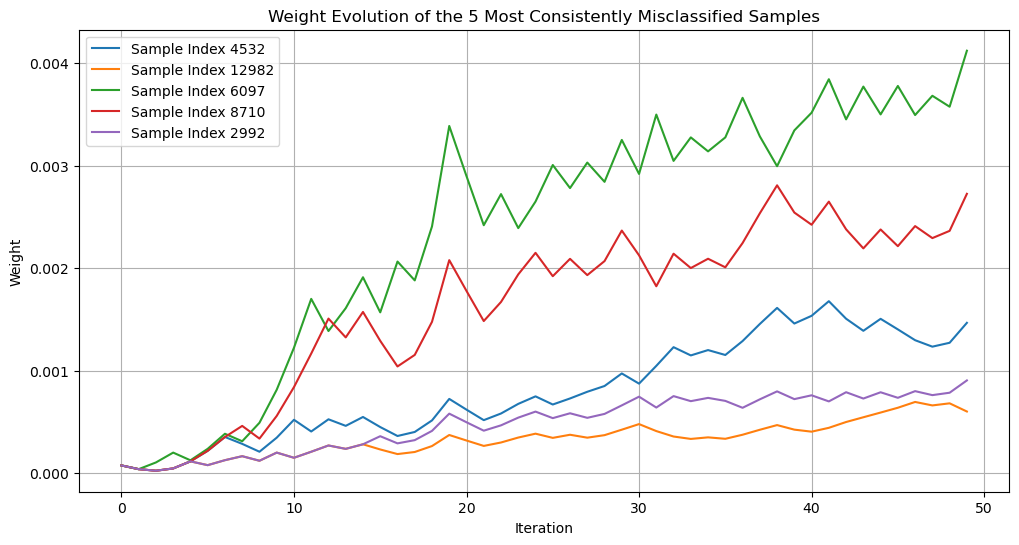
\includegraphics[width=\textwidth]{P01_3.png}
    \caption{Weight evolution of the 5 most consistently misclassified samples across AdaBoost iterations.}
    \label{fig:1_3}
\end{subfigure}
\hfill
\begin{subfigure}[b]{0.43\textwidth}
    \centering
    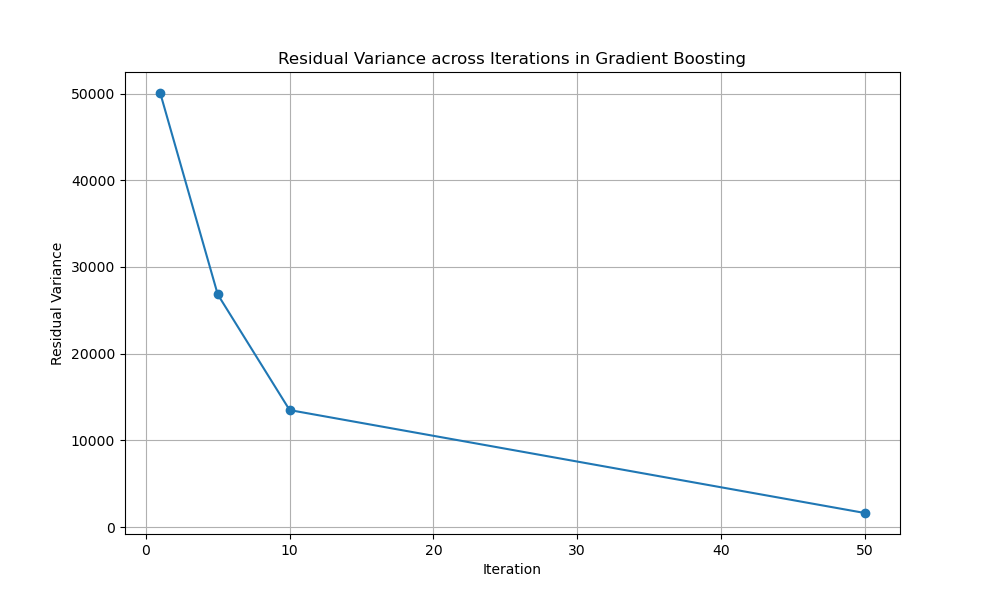
\includegraphics[width=\textwidth]{P01_4.png}
    \caption{Residual variance across Gradient Boosting iterations.}
    \label{fig:1_4}
\end{subfigure}
\end{figure}

\questionheader{Phase 2: Subspace \& Clustering}

\textbf{2.5 PCA vs. Linear Autoencoders}
\begin{solution}
PCA is implemented through SVD on the standardized data matrix, and the bottleneck size of the linear autoencoder is set equal to the PCA dimension. PCA retains 95\% variance with \textbf{4} components. PCA reconstruction MSE = \textbf{0.0469}. Linear autoencoder reconstruction MSE = \textbf{0.0546}. Both give similar low-error reconstructions, which empirically shows that the linear AE learns nearly the same subspace as PCA.
\end{solution}

\textbf{2.6 GMM Latent Clustering}
\begin{solution}
The final dense feature vectors are extracted from the Assignment 2 CNN after removing the classification head, and a GMM is fit on these embeddings. The Adjusted Rand Index is \textbf{0.2808}. This indicates that the latent features contain some class structure, but the unsupervised clusters are still far from perfectly aligned with the true disease labels.
\end{solution}

\questionheader{Phase 3: Deep Generative Models}

\textbf{3.7 ELBO Implementation}
\begin{solution}
The VAE is trained by optimizing the ELBO,
\[
\mathcal{L} = \mathcal{L}_{\text{recon}} + \beta\,D_{KL}(q(z|x)\|p(z)),
\]
with a short $\beta$ warm-up. At the final epoch, total loss = \textbf{16.0327}, reconstruction loss = \textbf{0.0327}, and KL loss = \textbf{16.0000}. The KL term dominates after the warm-up reaches $\beta=1$.
\end{solution}

\textbf{3.8 VAE vs. Simple DCGAN}
\begin{solution}
Samples are generated using \verb|model_vae.sample(16)| and \verb|model_gan.generate(16)|. Fig.~\ref{fig:3_8} shows samples from both models. The VAE outputs are smoother and blurrier, while the DCGAN outputs are visually sharper. This is expected because the VAE optimizes a likelihood-style reconstruction objective averaged over many valid outputs, whereas the GAN directly learns to fool the discriminator and therefore produces visually crisper samples.
\end{solution}

\textbf{3.9 Frechet Inception Distance (FID)}
\begin{solution}
FID is computed by passing real and generated images through frozen \texttt{inception\_v3} and then applying
\[
\|\mu_r-\mu_g\|_2^2 + \mathrm{Tr}\left(\Sigma_r+\Sigma_g-2(\Sigma_r\Sigma_g)^{1/2}\right).
\]
Using real APTOS Class-4 images and generated GAN samples, the feature shapes are \textbf{(295, 2048)} and \textbf{(500, 2048)} respectively. The computed FID score is \textbf{384.2104}.
\end{solution}

\textbf{3.10 Batch Normalization \& Mode Collapse}
\begin{solution}
All \verb|nn.BatchNorm2d| layers in the generator are replaced by \verb|nn.Identity()| and the model is retrained. After removing BatchNorm from the APTOS generator, the generated samples show much lower diversity and stronger collapse patterns, as seen in Fig.~\ref{fig:3_10}. BatchNorm stabilizes feature statistics across mini-batches; without it, the generator updates become less stable and it is easier for the model to collapse to a few repeated modes.
\end{solution}

\begin{figure}[H]
\centering
\begin{subfigure}[b]{0.90\textwidth}
    \centering
    
\includegraphics[width=\textwidth]{P03_8.png}
    \caption{VAE (top) vs.\ DCGAN (bottom) on PlantVillage.}
    \label{fig:3_8}
\end{subfigure}

\vspace{0.5em}

\begin{subfigure}[b]{0.90\textwidth}
    \centering
    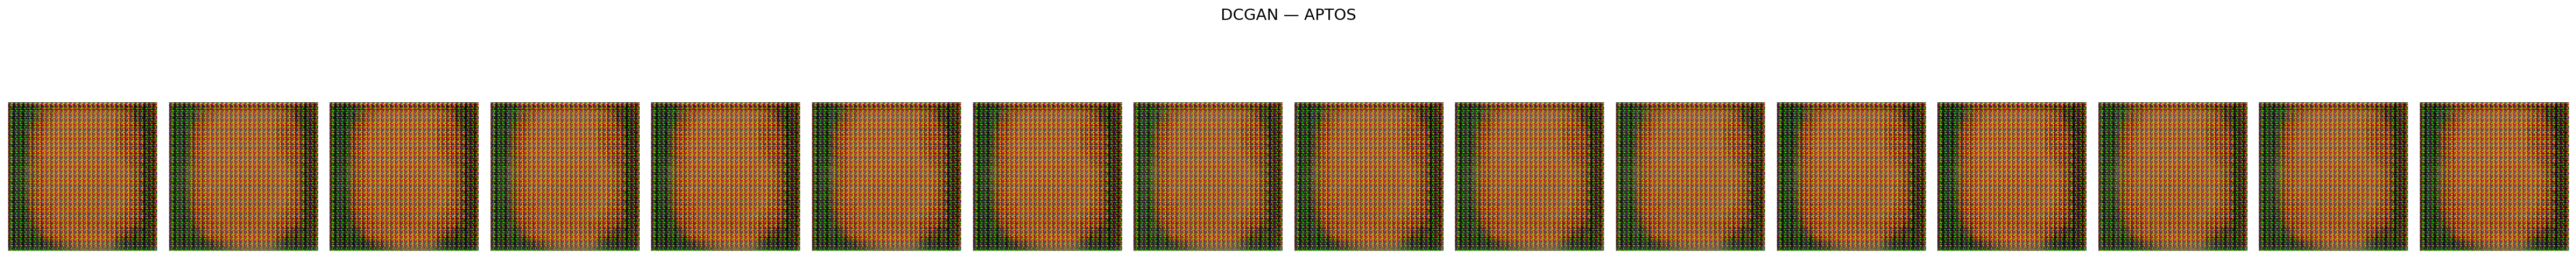
\includegraphics[width=\textwidth]{P03_10.png}
    \caption{APTOS GAN samples after removing Batch Normalization.}
    \label{fig:3_10}
\end{subfigure}
\end{figure}

\questionheader{Phase 4: Self-Supervised Learning via SimCLR}

\textbf{4.11 InfoNCE Loss}
\begin{solution}
The SimCLR pipeline uses two random augmented views per image with \verb|RandomResizedCrop|, \verb|RandomHorizontalFlip|, \verb|ColorJitter|, and \verb|RandomGrayscale|. The encoder and projection head are trained using the normalized temperature-scaled InfoNCE loss. Final training loss at Epoch 30/30 = \textbf{2.2675}. Final validation loss at Epoch 30/30 = \textbf{3.5570}.
\end{solution}

\textbf{4.12 Linear Evaluation Protocol}
\begin{solution}
For linear evaluation, the ResNet18 encoder weights are frozen and only a single \verb|nn.Linear| head is trained on top. With the frozen SimCLR encoder and a linear probe, the test cross-entropy loss is \textbf{11.9454}. For comparison, the fully supervised CNN gives test cross-entropy loss \textbf{0.2865}. The supervised CNN from Assignment 2 therefore remains much stronger on this dataset, showing that the learned self-supervised representation is not yet as discriminative as the fully supervised one.
\end{solution}

\questionheader{Phase 5: Policy Gradient Theorem}

\textbf{5.13 REINFORCE Implementation}
\begin{solution}
The policy is a small MLP that outputs the probability of purifier ON/OFF, and it is updated using the REINFORCE rule
\[
\nabla_\theta J(\theta) \approx \sum_t \nabla_\theta \log \pi_\theta(a_t|s_t)\,G_t.
\]
The state is the past 24 hours of meteorological data flattened into one vector, and rewards include a small energy penalty for purifier ON and a large health penalty when PM2.5 is high while the purifier stays OFF. The policy network was trained for \textbf{500} episodes. The episodic return trajectory is shown in Fig.~\ref{fig:5_13}.
\end{solution}

\begin{figure}[H]
\centering
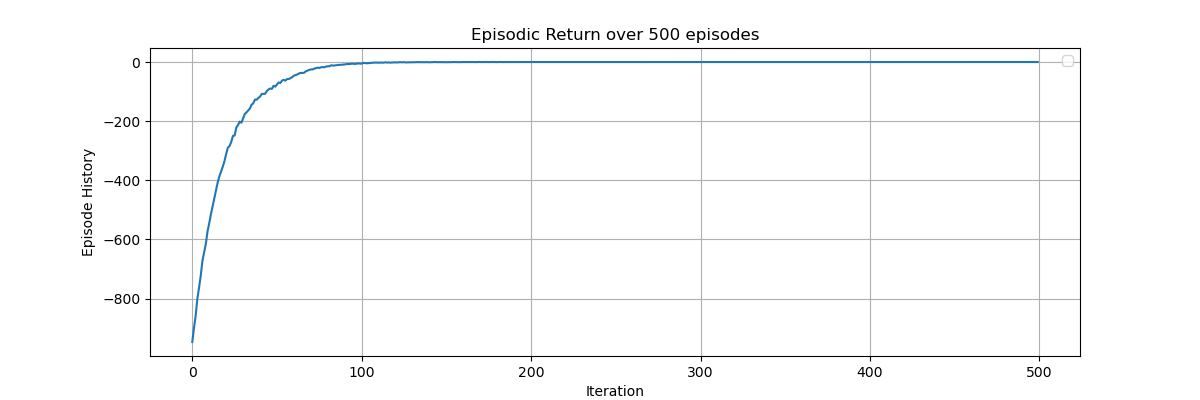
\includegraphics[width=0.72\textwidth]{P05_13.png}
\caption{Episodic return over 500 REINFORCE training episodes.}
\label{fig:5_13}
\end{figure}

\end{document}
